
\begin{figure}[h]
    \centering
    \vspace{-10pt}
    \captionsetup{font=small}
    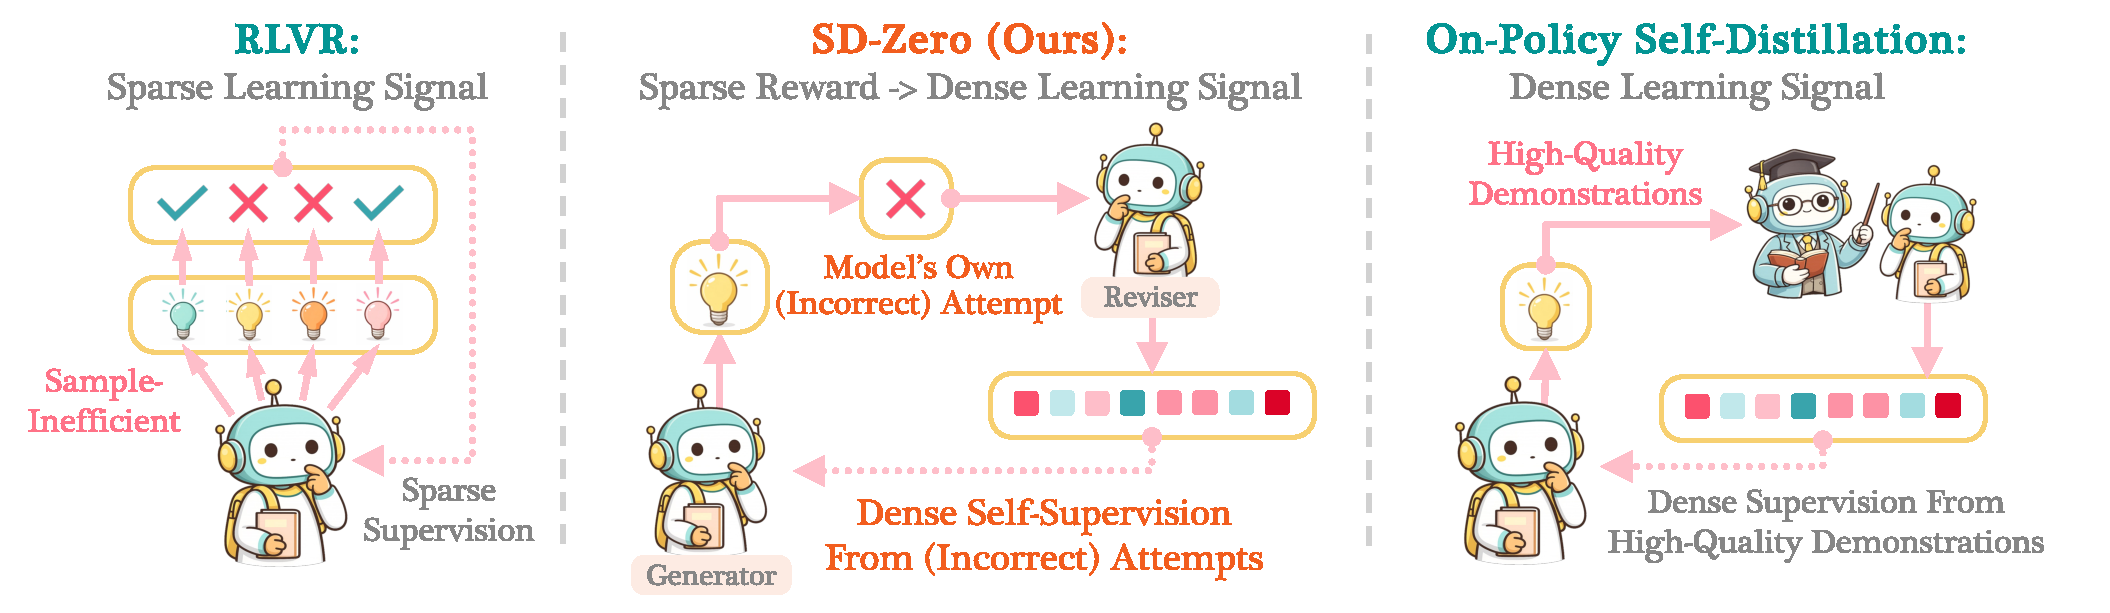
\includegraphics[width=0.95\textwidth]{figures/Picture0.pdf}
    \vspace{-5pt}
    \caption{
    % Reinforcement learning from verified rewards (RLVR) provides sparse learning signals; on-policy distillation relies on an external teacher to provide dense supervision. 
    We introduce \textbf{\ours{}}, an on-policy self-distillation paradigm where the teacher (\emph{reviser}) can condition on incorrect student (\emph{generator}) attempts.
    % that 
    % converts sparse rewards into dense self-supervision through self-revision feedback, without relying on high-quality demonstrations.
    % \danqi{This is my biggest confusion. This figure is about how self-distillation is different from RLVR and onpodi, but not about how your method is different from other self-distillation methods. There is no generator or reviser in the figure.}
    }
    \label{fig:starter}
\end{figure}

\section{Introduction}

% Story outline

% - Reinforcement learning - where we need to sample multiple responses and update based on a sparse reward.
% - Knowledge distillation - where a teacher needs to generate samples directly to train a student - can be bad for generalization
% - Recent - on policy self distillation, where a student provides dense supervision to itself when given access to ground truth chain of thought
% - Key disadvantage - we need access to ground truth chain of thought
% - Solution - if the student can critique its own responses when just given access to ground truth solutions, without chain of thought
% \liam{I wonder how much the intro should emphasize "reasoning" since I think it only works on non-thinking models?} 


% \yj{I think the background is currently too long (too much problem -> solution structure).
% SFT requires a lot of effort -> RL -> but RL rewards are sparse -> OPD -> but it requires a teacher -> ours (self-distillation).
% We should probably focus on the core motivation (e.g., we can do OPD with a self-teacher).}

%\looseness-1Reinforcement learning (RL) methods \citep{shao2024deepseekmath,Guo_2025,chen2025minimax,zheng2025group} have emerged as a dominant approach for improving reasoning performance of language models from sparse outcome supervision. In these methods, the model is trained with outcome supervision based on the correctness of its generated responses. Although effective, such supervision can be inefficient because it provides only weak \yh{sparse?} feedback for the intermediate reasoning steps within a response \citep{lu2025onpolicydistillation}. This has motivated growing interest in methods that can provide finer-grained supervision for generated responses.

% One promising alternative is on-policy distillation \citep{agarwal2024policy,lu2025onpolicydistillation,zhao2026self,shenfeld2026self}, where token-level supervision is provided on student-generated responses. Existing approaches typically rely on stronger external teachers or access to ground-truth solutions to provide such supervision. While these methods can substantially improve training efficiency, a key step toward more autonomous improvement is to reduce dependence on stronger external teachers or access to ground-truth solutions. This motivates the central question of our work:
% \begin{quote}
% Can we obtain token-level supervision from sparse outcome feedback, without access to a strong teacher or ground-truth solutions?
% \end{quote}

% \sk{Given changes in abstract, maybe we can rewrite first two paras of intro as follows:
% }\\

\looseness-1Reinforcement learning (RL) has become the dominant approach for post-training language models on reasoning tasks in verifiable settings such as math and coding \citep{shao2024deepseekmath,Guo_2025,chen2025minimax,zheng2025group}.
%\danqi{ and coding? cite}
These methods require only a binary reward, typically whether the final answer is correct, that makes them broadly applicable. However, a binary reward per response provides no information about which intermediate reasoning steps were sound. This sparse supervision makes training expensive: the model must discover good reasoning by comparing and contrasting many self-generated responses.

%\yj{This is probably a very minor point, but both OPD and SD are on-policy distillation methods. So maybe it's better could first introduce OPD as a method that usually relies on an external teacher, and then mention that, "more recently, there have been attempts to remove the external teacher. However, it still requires …" (something like this). But this is just a minor taxonomy point.}


\begin{figure}[t]
    \centering
    \captionsetup{font=small}
    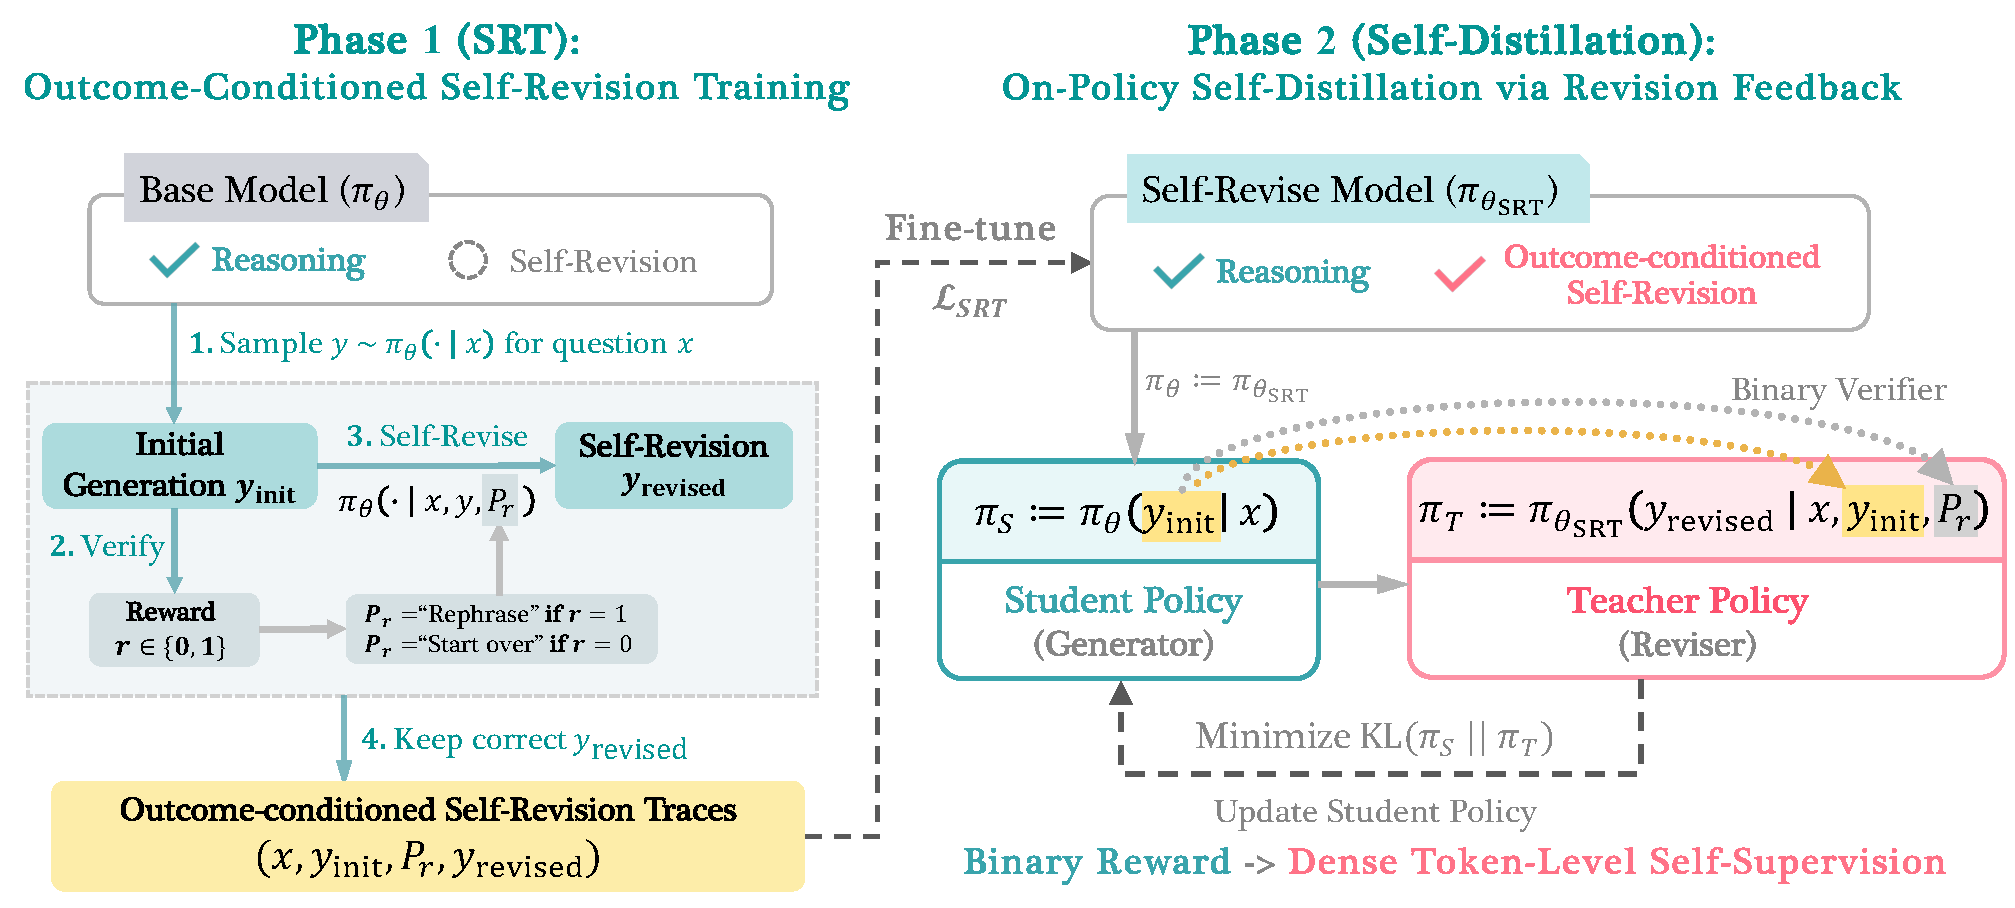
\includegraphics[width=\textwidth]{figures/Picture1.pdf}
    \caption{\textbf{Overview of \ours{}.} In \textbf{Phase 1 (\sft{})}, we collect 6K outcome-conditioned self-revision traces by sampling an initial response from the base model, prompting the model to self-revise its incorrect response, and keeping the correct self-revision. In \textbf{Phase 2 (\opsd{})}, we conduct on-policy self-distillation with the self-revise (\sft{}) model acting as both student and teacher: the \textit{student} generates an on-policy response, and the \textit{teacher} generates a revised version conditioned on that response and its outcome reward. Throughout the \opsd{} phase, the model bootstraps performance through internalizing self-revision behavior. See \Cref{alg:pipeline} for details.
    % \liam{I'm very confused by this diagram - and unless I'm being dumb, I feel like the OPSRD loss setup might not make total sense (notationally)?}
    % \yh{make things consistent with section 2}
    % \\\yj{I'm confused of what are these check signs? So to my understanding, regardless of correctness, the model self-revises the response and filters out only the correct revised response? Also, it's hard to get the fine-tuning objective with this "self-revision traces" and that we are "minimizing" this KL. Finally, I think notations are not consistent with the explanation ($z$ and $y_{revisied}$)?}
    % \danqi{What is $\theta^*$? Do generator and reviser always share weights?}
    }
    
    \label{fig:main-figure}
\end{figure}




\looseness-1Distillation methods provide a more sample-efficient alternative by converting supervision into token-level feedback on student-generated responses. \emph{On-policy distillation} methods \citep{agarwal2024onpolicy,gu2024minillm,boizard2024uld,minixhofer2025cross,lu2025onpolicydistillation} assume access to an external stronger teacher that can provide token-level feedback on the student's responses. More recent \emph{self-distillation} methods, including OPSD \citep{zhao2026self}, SDFT \citep{shenfeld2026self}, and SDPO \citep{hubotter2026reinforcement}, remove the external teacher but still require high-quality demonstrations that are much better than the model's responses.
These demonstrations are typically assumed to come from an external teacher (OPSD, SDFT) or repeated generation and filtering from the model itself (SDPO) \footnote{See \Cref{tab:comparison} for a detailed comparison of post-training methods.}. Collecting such supervision can be unavailable or prohibitively expensive to collect. This raises the central question of our work:

\begin{quote}
    Can the model condition its own initial attempts (possibly incorrect) and their sparse rewards, and provide improved dense supervision to itself?
\end{quote}






%\ap{we can even condition on incorrect response}
%\citep{agarwal2024policy,gu2024minillm,boizard2024uld,minixhofer2025cross,lu2025onpolicydistillation,zhao2026self,shenfeld2026self}. On-policy distillation
%At each token position, the student is trained to match the predictions of a teacher. However, these approaches typically require either token-level supervision from a stronger teacher.. 

% \begin{quote}
%     Can we obtain token-level supervision from sparse outcome feedback, without access to a strong teacher or ground-truth solutions?
%     \ap{}
% \end{quote}
 
\looseness-1\textbf{\method{} (\ours{}):}
Our method is built around a single model that plays two roles: a \textit{generator} and a \textit{reviser}. As a generator, the model produces candidate responses to a given question. As a reviser, the same model is conditioned on its own response and reward, and either {corrects} an \emph{incorrect} response or {rephrases} a \emph{correct} one.

%\danqi{why do we need to rephrase a correct one? is it possible the answer is correct but intermediate solution is wrong?} \danqi{Maybe you will make it clearer later but i still feel demonstration / answer are not so well defined and the verifier is only applied to the answer.}

\looseness-1\ours{} proceeds in two phases. In the first phase, we collect self-revision traces by sampling responses, checking for correctness, and prompting the model to revise incorrect ones. We retain only traces where revision succeeds. We fine-tune on these filtered traces, a procedure we call Self-Revision Training (\sft{}).
In the second phase (self-distillation), we use the reviser as a teacher to provide token-level supervision over the generator's responses, thereby transforming outcome-level reward into dense token-level supervision.

% Our method instantiates a single model in two roles: a \textit{generator} and a \textit{reviser}. As a generator, the model produces candidate responses to a given question. As a reviser, the same model is conditioned on its own response and its correctness, and either \textit{revises} an incorrect response or \textit{rephrases} a correct one. \ours{} then uses the reviser as a teacher to provide token-level supervision over the generator’s sampled responses, thereby converting sparse outcome feedback on the responses into dense token-level feedback. To enable this behavior, \ours{} begins with an initial training phase in which an off-the-shelf model is trained to perform both revision and rephrasing on its own sampled responses.\ap{make sure intro is self-contained}

\textbf{Key Findings.} Applying \ours{} on Olmo and Qwen models on math and code reasoning datasets shows the following: 
% \citep{openr1}\danqi{why cite OpenR1 here?} 
\begin{itemize}
    \item \looseness-1\textbf{Phase 1 (\sft{}) alone outperforms all baselines on the same data budget.}
    Training on 6K self-generated revision traces improves average accuracy by 7.8\% for \qwen{} and 9.2\% for \olmo{} (\Cref{tab:main_results}). 
    
    % \item \looseness-1\textbf{Phase 2 (\opsd{}) is essential for the major efficiency gains of \ours{} at both training and inference time.}
    % Models trained only with \sft{} tend to produce excessively long and verbose responses. In contrast, \opsd{} teaches the model to internalize its \textit{revision} behavior, enabling it to generate stronger responses directly as the \textit{generator}. As a result, responses after \opsd{} are approximately $2\times$ shorter than those from \sft{} (\Cref{fig:self-revision}). Beyond this efficiency benefit, \opsd{} also delivers an additional $2.7\%$ gain for \qwen{} and $1.2\%$ for \olmo{} over \sft{}, bringing the total improvement over the base models to $10.5\%$ and $10.4\%$, respectively.
    % \emph{Crucially}, this second phase is what makes \ours{} highly sample-efficient during training: \opsd{} requires only a single response per question, whereas the \sft{} phase must collect multiple sampled responses to construct revision traces. We provide a more detailed analysis in \Cref{sec:distillation-results}.
    
    \item \looseness-1\textbf{Phase 2 (\opsd{}) is critical for the training and inference efficiency of \ours{}.}
     \sft{} trained model produces overly long responses. \opsd{} trains the model to internalize its \textit{revision} behavior and generate stronger answers directly as the \textit{generator}, reducing response length by roughly $2\times$ (\Cref{fig:self-revision}). It also improves performance beyond \sft{}, yielding an additional $2.7\%$ gain for \qwen{} and $1.2\%$ for \olmo{}, for total gains of $10.5\%$ and $10.4\%$ over the base models. \emph{Importantly}, \opsd{} is also what makes \ours{} training sample-efficient during training: it requires only one response per question, whereas \sft{} must sample multiple responses to construct revision traces (\Cref{sec:distillation-results})
    %\opsd{} yields an additional $2.7\%$ gain for \qwen{} and $1.2\%$ for \olmo{} beyond \sft{}, resulting in total gains of $10.5\%$ and $10.4\%$, respectively, over the corresponding base models. 

    % \\\sk{For phase 2 bullet, I think we should lead with the problem phase 1 caused (very long generations) that phase 2 fixes. I'm worried if a lazy reviewer sees the 2.7\% gains first, they might conclude that Phase 2 offers marginal improvement / isn't needed. But if they first read that phase 2 compresses verbose revision into efficient generation, I think the story would read as "phase 1 unlocks the capability, phase 2 makes it practical"}


    \item \looseness-1\textbf{\ours{} enables iterative self-evolution through regular teacher synchronization.}
    Because training also improves the model’s revision capability, the updated model can serve as the reviser teacher in subsequent rounds of \opsd{}. After one epoch of \opsd{}, synchronizing the teacher with the updated model yields a further performance gain of at least $3\%$ (\Cref{fig:evolution}), suggesting that \ours{} can continue to improve over multiple rounds of \opsd{}.
    % \item \looseness-1\textbf{Phase 2 (\opsd{}) further improves average accuracy while reducing response length.}
    % This phase yields an additional 2.7\% gain for \qwen{} and 1.2\% for \olmo{} beyond \sft{}, resulting in total gains of 10.5\% and 10.4\%, respectively, over the corresponding base models. Notably, \ours{} produces responses that are approximately 2$\times$ shorter than those from \sft{} (\Cref{fig:self-revision}), suggesting that the model internalizes its \textit{revision} behavior and generates stronger responses as the \textit{generator}.
    % \item 
    % \textbf{Phase 2 (\opsd{}) is critical to realize the full benefits of \ours{}:} Although the \sft{} phase delivers most of the improvement over the base model, it also causes the model to generate responses that are nearly $2\times$ longer than those of the baselines. \opsd{} is essential for recovering efficiency: it significantly shortens responses while still providing additional accuracy gains of $2.7\%$ on \qwen{} and $1.2\%$ on \olmo{} beyond \sft{}. Importantly, this second phase remains highly generation-efficient, requiring only one response per question during training, unlike \sft{} that relies on generation of multiple samples. We provide further analysis in \Cref{sec:distillation-results}.
    % \item \looseness-1\textbf{\ours{} enables iterative self-evolution through regular teacher synchronization.}
    % Because training also implicitly improves the model’s revision capability, the updated model can serve as the new reviser teacher in subsequent rounds of self-distillation. After one epoch of \opsd{}, synchronizing the teacher with the updated model yields a further performance gain of at least 3\% (\Cref{fig:evolution}), suggesting that the model can continue to self-evolve with teacher synchronization through multiple rounds of \opsd{}.
    %, indicating that the model internalizes the self-revision behavior of the revision phase into more directed first-attempt reasoning rather than explicit backtracking.
    %A second \opsd{} phase with a synchronized teacher yields further gains after the first phase (\Cref{fig:evolution}), suggesting that  
    %phase instills a self-improvement loop that persists across multiple distillation iterations. 
    %[todo: reword ``synchronization'' part?]
\end{itemize}


%\emph{In comparison}, rejection fine-tuning (RFT) learns only from the model's correct responses, discarding incorrect attempts entirely, while RL methods such as GRPO improve by comparing and contrasting multiple sampled responses under binary rewards, without learning how to transform a weak response into a stronger one. In contrast, 
% \looseness-1Overall, \ours{} shows that a model can bootstrap  self-revision behavior from binary rewards and convert into dense self-supervision.


% \ap{TODO: need a finishing paragraph here}

% \sk{feel free to revise the following draft}
% \sk{
% Key findings:
% \begin{itemize}
%     \item \textbf{Phase 1 (SRT) alone outperforms all baselines on the same data budget.}
%     Training on approximately 5K self-generated revisions traces improves average avg@16 accuracy by 7.8\% for Qwen3-4B-Instruct and 9.2\% for OLMo-3-7B-Instruct (Table 1) [todo: add link]. 
%     \item \textbf{Phase 2 (OSRD) further improves accuracy while halving response length}. The distillation phase provides a 2.7\% gain for Qwen3-4B-Instruct and a 1.2\% gain for OLMo-3-7B-Instruct beyond SRT, for net gains of 10.5\% and 10.4\% over the respective instruct models (no training). Notably, the OSRD responses are approximately 2x shorter than SRT responses at equal or higher accuracy (Figure 2) [todo: link], indicating that the model internalizes the error-correction behavior of the revision phase into more directed first-attempt reasoning rather than explicit backtracking. 
%     \item \textbf{OSRD enables self-evolved reasoning through teacher synchronization [todo: reword ``synchronization'' part?]}. Because the trained OSRD model retains strong self-revision  capability, it can serve as its own teacher for subsequent rounds of distillation. A second OSRD phase with a synchronized teacher yields further gains after the first phase plateaus (Figure 3) [todo: add link], suggesting that SRT phase instills a self-improvement loop that persists across multiple distillation iterations. 
% \end{itemize}
% }
% \sk{todo: update key findings with GRPO/DAPO + sampling budget comparison to SRT}

% The remainder of the paper is organized as follows. \Cref{sec:method} presents \ours{} and details its two training phases (\Cref{sec:phase1,sec:phase2}). \Cref{sec:experiments} describes the experimental setup and reports results across a range of math and code benchmarks using \qwen{} \citep{yang2025qwen3technicalreport} and \olmo{} \citep{olmo2025olmo3}. \Cref{sec:discussion} provides extensive analysis and ablations examining how the models evolve during training. Finally, \Cref{sec:related} discusses related work and situates our approach in the broader literature.

% %\sk{decide if we want to include some outline of rest of paper layout ... and add appropriate links to relevant sections}
% \sk{

% Section 3 reports experimental results across eight math and code benchmarks (todo: cite which ones) and two model families.
% Section 4 analyzes the evolution of reasoning behavior from SRT to OSRD and prseents ablation studies.
% Section 5 discusses related work.
% }




% Thus, a key question is how should we convert the sparse outcome feedback to dense feedback for the model. Here, we propose a training pipeline where the 




% Recent language models have achieved remarkable performance on reasoning-intensive tasks such as mathematics and coding, driven largely by three families of training algorithms: supervised fine-tuning, knowledge distillation, and reinforcement learning. Supervised fine-tuning and distillation can provide dense token-level supervision by training on full reasoning traces, but both rely on access to high-quality trajectories and can be brittle when the provided traces are misaligned with the student model’s knowledge, reasoning style, or capabilities. As a result, reinforcement learning from outcome supervision has emerged as a dominant strategy for improving reasoning: the model samples multiple candidate solutions and receives reward based on whether the final answer is correct. However, this form of training is inherently sample-inefficient, since the learning signal is sparse and only weakly localizes which parts of a reasoning trace should be reinforced or corrected.

% A natural alternative is to combine the strengths of both paradigms: preserve the on-policy nature of reinforcement learning, while recovering denser supervision from the model’s own sampled trajectories. Recent work on on-policy distillation moves in this direction by using stronger teacher feedback or ground-truth chain-of-thought traces to provide process-level supervision for the model’s own generations. Yet these approaches require access to teacher rationales or gold reasoning traces, which are often unavailable in realistic settings. This leaves open a central question: can a model improve from outcome supervision alone, while still recovering dense learning signals that go beyond sparse reinforcement?


% Recent studies on language models have shown remarkable success in training them to achieve expert level performance on different reasoning benchmarks such as math and coding. Three primary algorithms have been proposed to train the models; supervised fine-tuning, knowledge distillation, and reinforcement learning. In supervised fine-tuning, we assume that we have access to ground truth reasoning traces and the model that we want to train needs to fit to the reasoning trace. However, such form of training can hurt the model performance, due to gaps in the knowledge of the model and the style of the reasoning traces. 

% To mitigate, reinforcement learning has become a dominant strategy to train the models. In this paradigm, multiple reasoning traces are sampled from the model itself and the traces that lead to the correct solution receive positive reinforcement, and contrasted against traces that lead to incorrect solution. Although such form of training has lead to extreme success in the community, one of the key issues of reinforcement learning is that it is sample inefficient, and because of sparse feedback signal, we can only hope that the model learns only when we hit the positive reasoning trace per question. A mitigation instead is on-policy distillation, where a teacher provides denser supervision to generations from the model. However, this assumes access to a teacher that can provide the right feedback. Thus, a key question in the community is whether a model can self-improve itself.

